\documentclass[a4paper,12pt]{report}
\usepackage[utf8]{inputenc}
\usepackage[T1]{fontenc}
\usepackage[english]{babel}
\usepackage{lmodern}

%Figure progressive enumeration
\usepackage{chngcntr}
\counterwithin{figure}{chapter}
\counterwithin{table}{chapter}

%package used to enumerate figures
\usepackage[labelfont=bf]{caption}

%hyperref for interactive PDF index
\usepackage[bookmarks, colorlinks, breaklinks]{hyperref}
\hypersetup{linkcolor=black, citecolor=black, filecolor=black, urlcolor=black}

%Package required to use special symbols
\usepackage{amsmath, amssymb}

%Package required to use figures
\usepackage{graphicx}
%Include the bibliography in the table of contents
\usepackage{tocbibind}

%Package used to insert figures at the specified position
\usepackage{float}

%Our chapters must be called sections
\addto\captionsenglish{\renewcommand{\chaptername}{Section}}

\begin{document}

%Code for title page
\begin{titlepage}
\centering
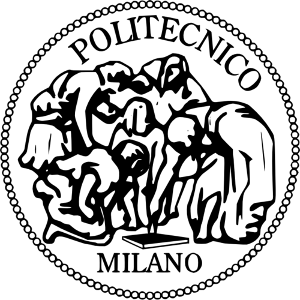
\includegraphics[width=0.30\textwidth]{./pictures/logo_poli}\par
	\vspace{1.8cm}
	{\Large {Embedded Systems} \par}
	\vspace{1.2cm}
	{\LARGE \textbf{mor1kx - Embedded CPU} \par}
	\vspace{0.5cm}
	{\LARGE \textbf{Write Back Cache Implementation \\
		Reference Manual} \par}
	\vspace{1.5cm}
	{\Large\itshape{Francesco Maio, Giovanni Scotti} \par}
	\vspace{2cm}
	\vfill
	% Bottom of the page
	{\large Document version: 1.0\par}
	{\large \today \par}
\end{titlepage}

%Make the table of contents
\tableofcontents

%INTRODUCTION
\chapter{Introduction}
\label{ch:Introduction}
\section{Purpose}
The Write Back Cache Implementation Reference Manual for the mor1kx embedded processor is intended to describe how the original architecture has been modified in order to provide the cache's write policy known as \textit{write-back}.

This document aims to supply an adequate knowledge to those developers and programmers, who have to change, adjust and enhance for any reason the related Verilog HDL code, making the understanding of what has been implemented much easier.

\section{Scope}
The mor1kx is an open source, Verilog implementation that is fully compliant with the OpenRisc architecture. In its \textit{Cappuccino} fashion, it offers a six stages pipeline with \textit{write-through} L1 caches.

The following sections deal with all the adjustments required to offer the more aggressive \textit{write-back} writing policy with respect to the \textit{Cappuccino} pipeline only.

\section{Definitions, Acronyms, Abbreviations}
\begin{description}
	\item[a.k.a:] Also Known As.
	\item[HDL:] Hardware Description Language.
\end{description}

\chapter{Original Functioning}
\label{ch:Original Functioning}
In this section the original operations of the mor1kx, concerning the write policy of the data cache, are briefly described to better understand which Verilog modules need to be modified and why.

\section{Write Through Implementation}
The followings are the relevant features offered before the changeover:
\begin{itemize}
	\item \textbf{\textit{write-through} write policy:} when a write occurs, data is written both to data cache and main memory;
	\item \textbf{no-write allocate:} on a write miss, data is directly written in main memory bypassing the data cache;
	\item \textbf{store buffer:} if enabled, during a store operation data is not only sent to the data cache, but also to the store buffer (a.k.a. write buffer). It is useful because bursts of writes are common. Moreover, it might prevent the processor from stalling.
\end{itemize}

The flow diagram in Figure \ref{wt_flow_diagram} depicts the series of procedures accomplished by the original implementation of the processor during read and write operations.

\begin{figure}[H]
	\begin{center}
		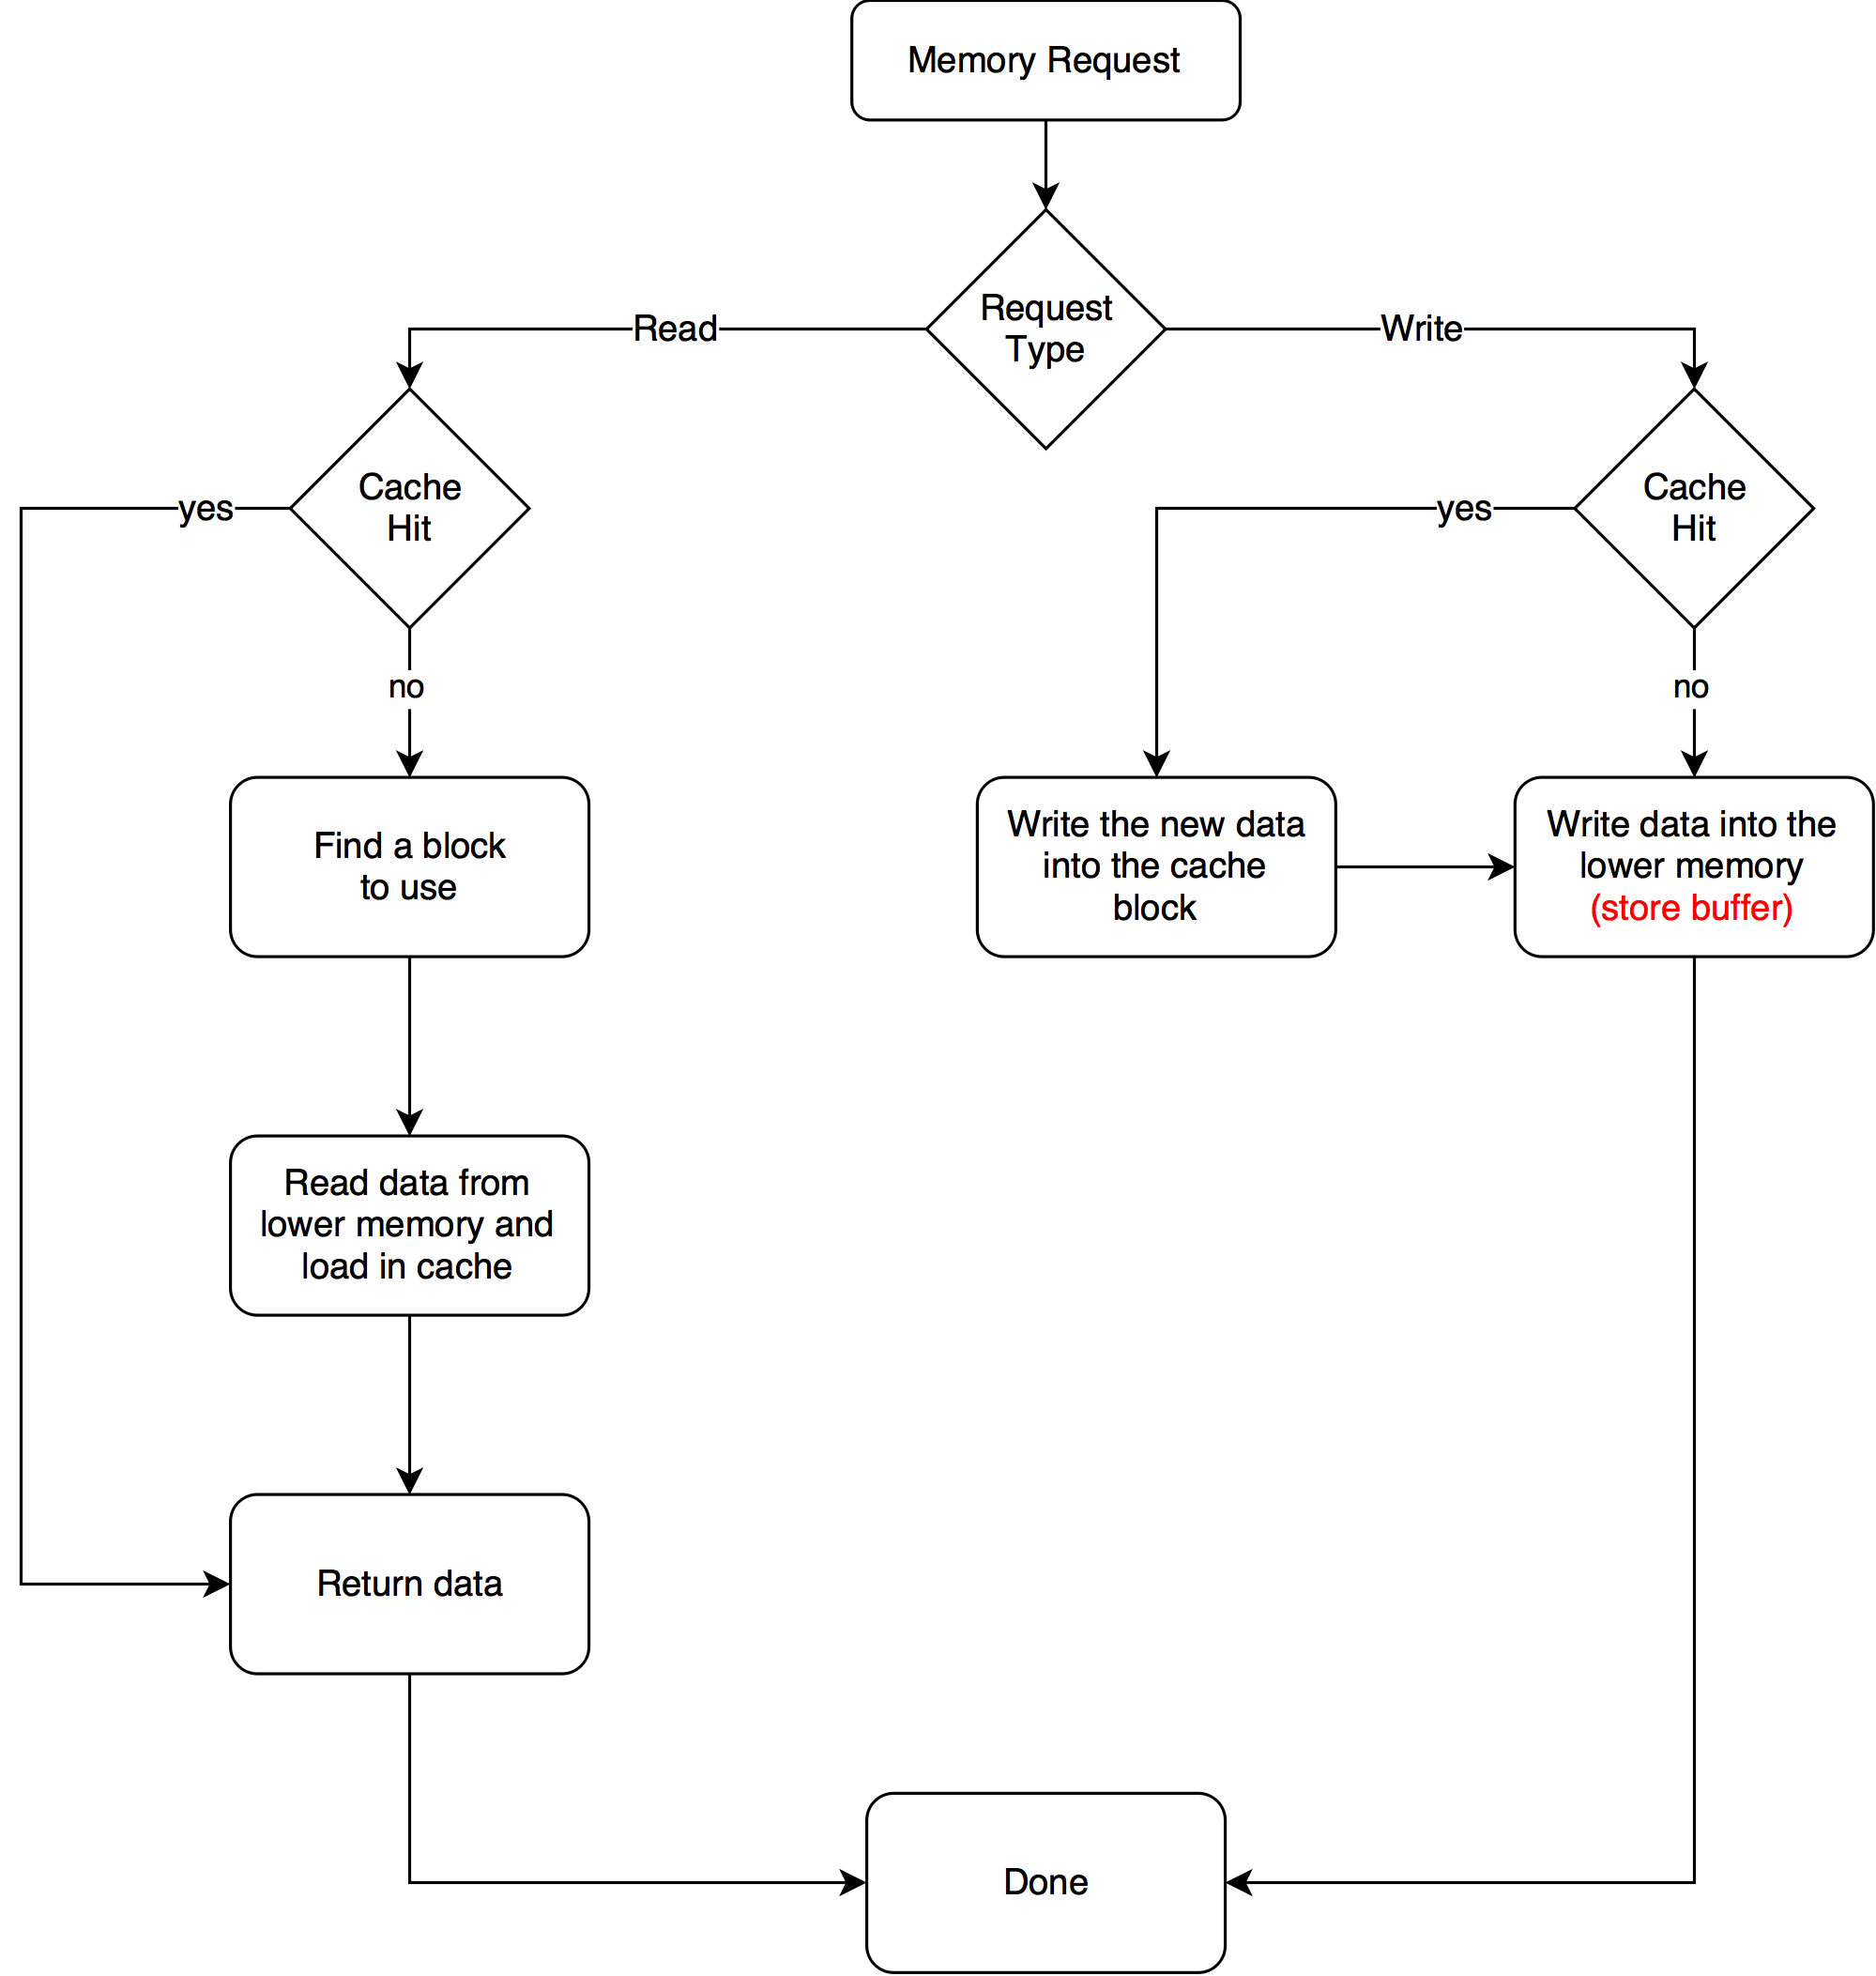
\includegraphics[width=\textwidth]{./pictures/cache_wt_flow.png}
		\caption{Flow diagram showing the original mor1kx \textit{write-through} working principle.}
		\label{wt_flow_diagram}
	\end{center}
\end{figure}

\section{System Configurations}
Different system configurations can be achieved by enabling and disabling the data cache and/or the store buffer. Both the modules are generated in the scope of the LSU module.

\begin{table}[H]
	\begin{center}
		\begin{tabular}{c | c | c}
			\hline
			Config. & Data Cache & Store Buffer \\
			\hline
			\hline
		    1 & Enabled & Enabled \\
		    \hline
		    2 & Enabled & None \\
		    \hline
		    3 & None & Enabled \\
		    \hline
		    4 & None & None \\
			\hline
		\end{tabular}
	\end{center}
	\caption{Potential system configurations of the original mor1kx implementation. The data cache and the store buffer are generated within the LSU \textit{Cappuccino} module.}
	\label{wt-system-configurations}
\end{table}

\chapter{Write Back Implementation}
\label{ch:Write Back Implementation}
\section{Overview}

\end{document}